\chapter{How to install LELAPE}
\section{Why Julia?}
The Julia language (\href{https://julialang.org}{https://julialang.org}] was released in 2012 as a possible solution the classical ``Two Languages' Problem"": a language easy to learn and develop in is usually slow and vice versa, so too often algorithms must be developped in one language and rewritten in another more efficient one. This language was specifically built to achieve speed, efficiency and clarity.

\section{How to install Julia}
%
Julia, an open software released with MIT license, can be downloaded and installed from \href{https://julialang.org/downloads/}{https://julialang.org/downloads/} for different operating systems and architectures. Depending on the system, the binary files will be installed (Microsoft Windows, macOS) or just uncompressed (GNU/Linux, FreeBSD). 

\begin{figure}
	\centering
	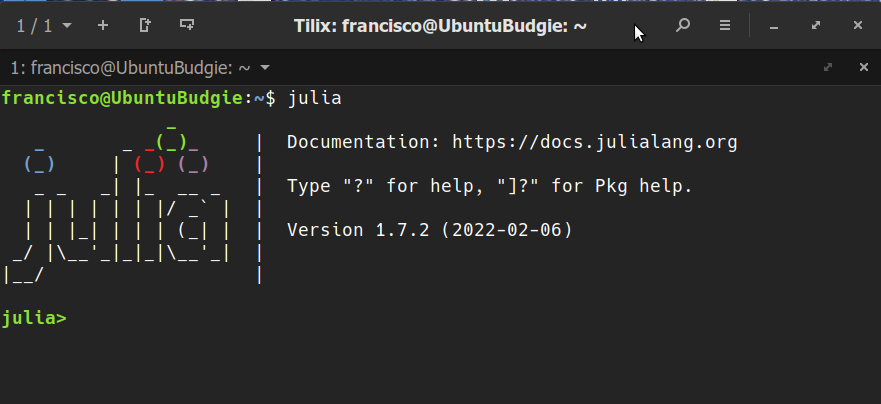
\includegraphics[width=0.65\textwidth]{fig/Julia_REPL}
	\caption{Example of the REPL's welcome screen for Julia on a machine running Ubuntu Budgie.}
	\label{Fig;JuliaREPL}
\end{figure}
%
If no additional tools is installed, Julia will be executed in a REPL as it is shown in Fig. \ref{Fig;JuliaREPL}. However, most of the users prefer to use the language in conjunction with IDEs or notebooks such as:`

\begin{itemize}
	\item \textbf{Visual Studio Code}: Popular IDE developed by Microsoft with plugins for Julia. It can be downloaded from \href{https://code.visualstudio.com/}{https://code.visualstudio.com/} and the plugins installed through the "Extensions" tool.
	%
	\item \textbf{Atom}: Just like VS Code, it is a general-purpose IDE with plugins for Julia.
	%
	\item \textbf{Jupyter}: Although it is typically used for Python, it is also appropriate for Julia. Indeed, Jupyther is an acronym for \textbf{Ju}lia-\textbf{Pyth}on-\textbf{R}. There are different ways of installing Jupyter. In systems with Microsoft Windows OS, the most simple way is to install Anaconda \href{https://www.anaconda.com/products/individual}{https://www.anaconda.com/products/individual}. Despite the fact of being designed for Python, Julia can be used as calculation engine. In GNU/Linux there are smaller packages to install Jupyter. For example, in Ubuntu the simple instruction \texttt{sudo apt install jupyter-notebook} will install the software in your computer. Later, it is necessary to install an additional package inside Julia but this will be studied a bit later.
	%
	\item \textbf{Pluto}: A notebook following the philosophy of Jupyter but specifically developed for Julia and easily extensible with JavaScript. Unlike the previous tools, it is installed inside Julia, not along with it. 
\end{itemize}
%
Atom, Jupyter and Pluto require the installation of additional packages. As Jupyter is probably the most popular tool, it is installed inside Julia REPL with the following instructions:

\vspace{1mm}
\begin{center}
	\texttt{using Pkg; Pkg.add("IJulia")}
\end{center}
\vspace{1mm}

This adds the software, which is launched as follows:

\vspace{1mm}
\begin{center}
	\texttt{using IJulia; notebook()} 
\end{center}
\vspace{1mm}

The other packages are installed following a similar procedure. 

\vspace{1mm}
\begin{center}
	\texttt{Using Pkg; Pkg.add("Pluto"); using Pluto; Pluto.run()}
\end{center}
\vspace{1mm}

There are other options if you prefer cloud computing. For  example, in spite of the fact that its primary use is running Python code, Google Colab is compatible with Julia language. For further information (and also learning a little Julia), you can read \href{https://colab.research.google.com/github/ageron/julia_notebooks/blob/master/Julia_for_Pythonistas.ipynb#scrollTo=GIeFXS0F0zww}{Julia for Pythonists} and use the \href{https://colab.research.google.com/github/ageron/julia_notebooks/blob/master/Julia_Colab_Notebook_Template.ipynb}{Julia Colab Template}. However, this solution is not recommended due to some problems at installing external packages as well as at loading data files. 

\section{Installing LELAPE}
LELAPE is built as a module. In Julia, a module is a set of elements such as variables, functions, etc. that can be loaded at will. The procedure is the following:
%
\begin{enumerate}
	\item Download the ZIP system from the website and decompress it. Also, you can clone the site with git.
	\item Find the folder where a file called LELAPE.jl is located.
	\item Copy the full path pointing to this folder (\texttt{PATH\_TO\_FOLDER}) and execute in REPL, Jupyter or the notebook you use the following command:
	
	\vspace{1mm}
	\begin{center}
		\texttt{push!(LOAD\_PATH, "PATH\_TO\_FOLDER")}
	\end{center}
	\vspace{1mm}	
	
	For example, if LELAPE.jl is found in \texttt{/home/johndoe/Download/LELAPE/src/}, the instruction is:
		
	\vspace{1mm}
	\begin{center}
		\texttt{push!(LOAD\_PATH, "/home/johndoe/Download/LELAPE/src")}
	\end{center}
	\vspace{1mm}	
	
	Thus, Julia knows where to find the module. \texttt{LOAD\_PATH} is a string vector that contains the list of folder where Julia must look up external libraries. \texttt{push!} is a function that adds a new element at the end of any vector, keeping the name. Therefore, we have just added a new entry to the original list.
	%
	\item Now, just launch LELAPE with the following instruction:
		
	\vspace{1mm}
	\begin{center}
		\texttt{using LELAPE}
	\end{center}
	\vspace{1mm}	
		
	After a few seconds to precompile the library, the functions are loaded. Fig. \ref{Fig:Loading_LELAPE} shows a practical example.
\end{enumerate}

\begin{figure}
	\centering

	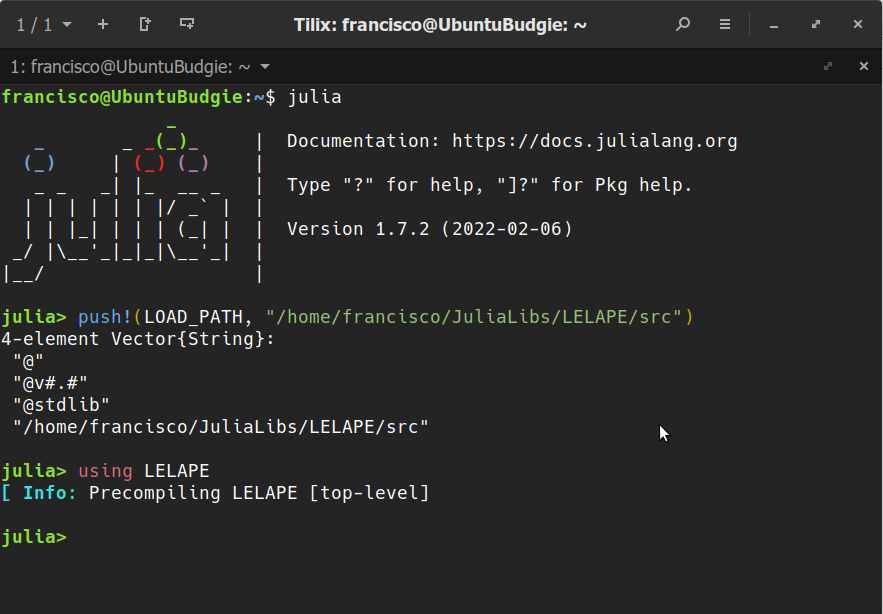
\includegraphics[width=0.65\textwidth]{fig/Loading_LELAP.png}
	\caption{How to indicate Julia where LELAPE is installed, and how to load it.}
	\label{Fig:Loading_LELAPE}
\end{figure}

\section{Recommended packages}
%
There are many Julia packages at the user's disposal that can be found on \href{https://juliapackages.com/}{https:// juliapackages.com/}. Some packages are extremely popular:
\begin{itemize}
	\item \textbf{Revise}: Useful for code developers since it allows reloading user functions without restarting Julia and losing information.
	\item \textbf{OhMyREPL}: Inteligent highlighting of elements in REPL. Figs. \ref{Fig;JuliaREPL} \& \ref{Fig:Loading_LELAPE} are using this package to show function names and strings.
\end{itemize}

Both are installed with \texttt{Pkg.add()}. 


Another interesting package to have is \textbf{DelimitedFiles}, which allows reading and writing CSV files. It is installed through:
	
\vspace{1mm}
\begin{center}
	\texttt{using Pkg; Pkg.add("DelimitedFiles")}
\end{center}
\vspace{1mm}	

This package is necessary to use the illustrative Jupyter notebooks that are provided along with LELAPE.
